

Os primeiros testes realizados, usando o sprite em front view (Figura \ref{fig:viduPablo}) para criação da animação de caminhada em side view, deixaram evidente uma grande dificuldade da ferramenta em manter o ambiente 2D, transformando o personagem para o 3D em um estilo cúbico, numa tentativa de replicar o estilo pixel art tridimensionalmente e mantendo as características físicas consistentes com a referência. Além disso, os resultados\footnote{\url{https://drive.google.com/drive/folders/10WGbLbvQspGPJlN8q57Up7GsKqN250aA?usp=drive_link}} adicionavam uma paisagem ao fundo e mostravam o personagem andando na diagonal, uma direção não presente no jogo desenvolvido. 

%fundo recorda o jogo minecraft

Porém, em um dos resultados, os erros de dimensão e direção foram corrigidos, formando uma animação 2D e realmente em side view. A Figura \ref{fig:viduComparaDimensao} apresenta a diferença entre os resultados, comparando um quadro do vídeo em 3D com um do em 2D.

\begin{figure}[htbp]
    \centering
    \caption{\small Comparação do resultado 3D e 2D gerado pelo Vidu}
    \label{fig:viduComparaDimensao}
    \begin{subfigure}{0.45\linewidth}
        \centering
        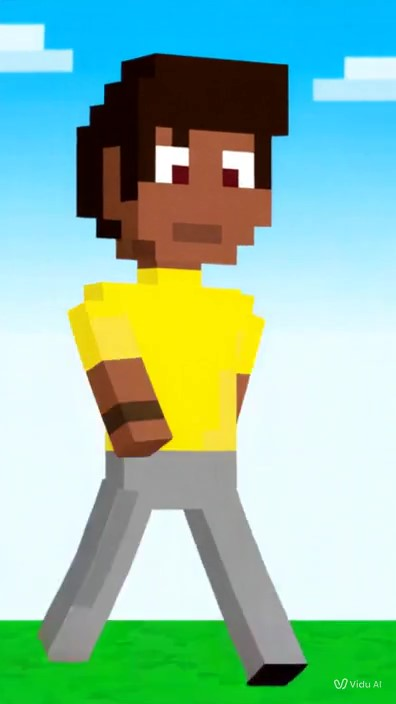
\includegraphics[width=0.8\linewidth]{figs/vidu/frame2.jpg}
        \caption{\small Frame da animação em 3D, com estilo cúbico e andando na diagonal}
        \label{fig:viduFrame3D}
    \end{subfigure}
    \begin{subfigure}{0.45\linewidth}
        \centering
        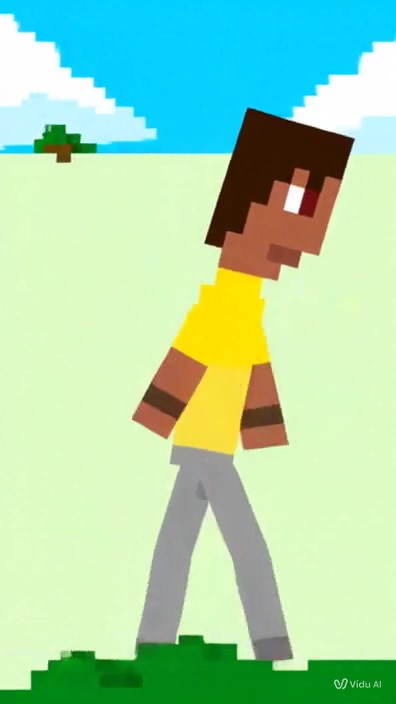
\includegraphics[width=0.8\linewidth]{figs/vidu/frame3.jpg}
        \caption{\small Frame da animação em 2D, andando em side view}
        \label{fig:viduFrame2D}
    \end{subfigure}
    \legend{\small Fonte: Elaborada pela autora, utilizando a ferramenta Vidu.}
\end{figure}

Apesar disso, a nova imagem formada para o personagem em side view possuía a cabeça muito quadrada e, mesmo que o design ainda fosse em pixel art, a animação deformava esse estilo, da mesma forma que aconteceu com a ferramenta Animated Drawnings (descrita na Seção \ref{s.sketchLab}). Outro detalhe observado nesse vídeo específico foi que, durante a animação de andar, o personagem nem sempre dobra a perna ou, quando dobra, é muito pouco, formando uma movimentação que causa estranheza ao olhar. A postura inclinada para frente, o movimento brusco do braço e a quantidade variável de movimentação do mesmo contribuem para esse estranhamento. 

Para entender a causa de apenas um dos testes produzir o vídeo em 2D, analisou-se a metodologia de cada um deles. A principal diferença encontrada foi a estrutura do prompt textual. Como a plataforma mostra de exemplo (Figura \ref{fig:viduPromptExemplo}), nos vídeos em 3D, a tag da imagem de referência foi usada como sujeito da frase (Figura \ref{fig:viduPrompt3d}). Enquanto no vídeo em 2D, a instrução foi mais imperativa e descritiva, sem considerar a tag como uma palavra a ser usada e apenas como forma de marcar que a imagem foi anexada (Figura \ref{fig:viduPrompt2D}). Baseado nisso, levanta-se a hipótese de que, ao não tratar a imagem como um sujeito imutável, a IA teve maior liberdade para reinterpretar o personagem e criar um novo sprite 2D em side view, em vez de apenas rotacionar a imagem de referência, o que mantinha características do sprite em front view e adicionava profundidade para parecer parcialmente de lado.

\begin{figure}[htbp]
    \centering
    \caption{\small Exemplo de prompt mostrado no Vidu}
    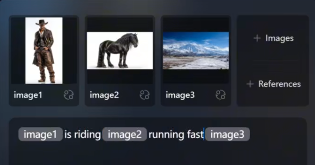
\includegraphics[width=0.6\linewidth]{figs/vidu/promptEx.PNG}
    \label{fig:viduPromptExemplo}
    \legend{\small Fonte: Elaborada pela autora.}
\end{figure}

\begin{figure}[htbp]
    \centering
    \begin{minipage}{0.45\textwidth}
    \centering
    \caption{\small Prompt que gerou vídeo em 3D no Vidu}
    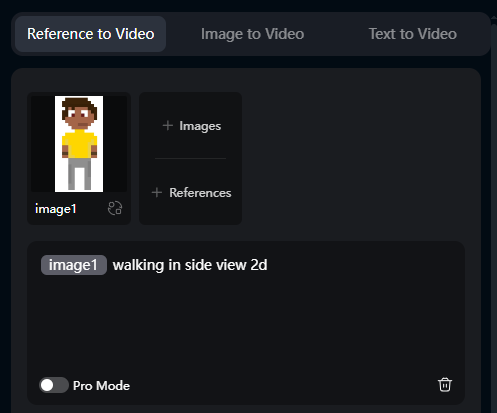
\includegraphics[width=0.9\linewidth]{figs/vidu/prompt2.PNG}
    \label{fig:viduPrompt3d}
    \legend{\small Fonte: Elaborada pela autora.}
    \end{minipage}\hfill
    \begin{minipage}{0.45\textwidth}
    \centering
    \caption{\small Prompt que gerou vídeo em 2D no Vidu}    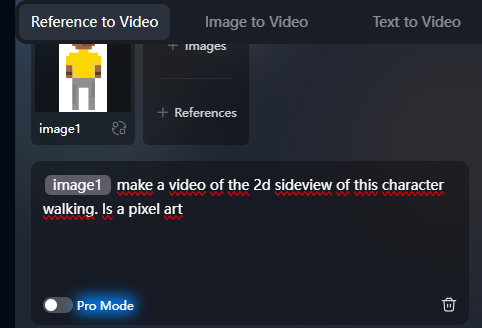
\includegraphics[width=0.9\linewidth]{figs/vidu/prompt3.PNG}
    \label{fig:viduPrompt2D}
    \legend{\small Fonte: Elaborada pela autora.}
    \end{minipage}\hfill
    
\end{figure}

Comparando tudo, foi notado que o vídeo em 2D aparentava possuir mais frames com partes borradas em relação às animações em 3D. Para confirmar essa teoria, os vídeos foram transformados em sprite sheet, com a ferramenta ezgif\footnote{https://ezgif.com/} (transforma vídeo em gif, e gif em sprite sheet), e foi feita uma análise quadro a quadro, verificando quais frames apresentavam uma grande deformação e nenhuma deformação.

\begin{table}[htbp]
    \centering
    \caption{Análise quantitativa de frames com deformação nos vídeos gerados pelo Vidu}
    \label{tab:viduDeformacoes}
    \begin{tabular}{l c c c}
        \toprule
        \textbf{Nível de deformação} & \textbf{Vídeo 1 (3D)} & \textbf{Vídeo 2 (3D)} & \textbf{Vídeo 3 (2D)} \\
        \midrule
        Deformação grave (\%) & 7,32\% & 12,2\% & \textbf{36,59\%} \\
        (Frames) & 3 &  5 & \textbf{15} \\
        \midrule
        Deformação leve (\%) & 48,78\%  & 41,46\% & 39,02\% \\
        (Frames)& 20 & 17 & 16 \\
        \midrule
        Sem deformação (\%) & 43,9\% & 46,34\% & \textbf{24,39\%} \\
        (Frames)&18 & 19 & \textbf{10}\\
        \midrule
        \textbf{Total (\%)} & 100\% & 100\% & 100\%  \\
        \textbf{(Frames)} & 41 & 41 & 41 \\
        \bottomrule
    \end{tabular}
    \legend{\small Fonte: Elaborada pela autora.}
\end{table}

A Tabela \ref{tab:viduDeformacoes} comprova a hipótese. O vídeo gerado em 2D, apresentou uma taxa de frames com deformação grave (partes muito borradas) quase duas vezes maior que a taxa somada dos vídeos em 3D. Consequentemente, o número de frames sem deformação foi quase metade em comparação com as versões 3D. As Figuras \ref{fig:viduNiveisDeformacao1} a \ref{fig:viduNiveisDeformacao3} apresentam exemplos visuais que definem cada categoria de deformação utilizada na análise de cada um dos vídeos.

\begin{figure}[htbp]
    \centering
    \caption{\small Quadros do Vídeo 1 (3D) em cada um dos níveis de deformação}
    \label{fig:viduNiveisDeformacao1}
    \begin{subfigure}{0.32\linewidth}
        \centering
        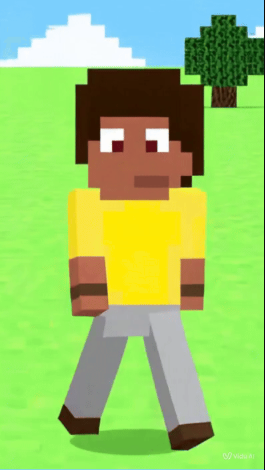
\includegraphics[width=0.8\linewidth]{figs/vidu/1sem.png}
        \caption{\small Quadro classificado como sem deformação}
        \label{fig:viduDeformacao1Sem}
    \end{subfigure}
    \begin{subfigure}{0.32\linewidth}
        \centering
        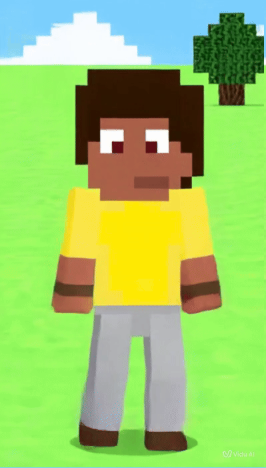
\includegraphics[width=0.8\linewidth]{figs/vidu/1leve.png}
        \caption{\small Quadro com deformação leve (borda da perna com pequenas ondulações)}
        \label{fig:viduDeformacao1Leve}
    \end{subfigure}
    \begin{subfigure}{0.32\linewidth}
        \centering
        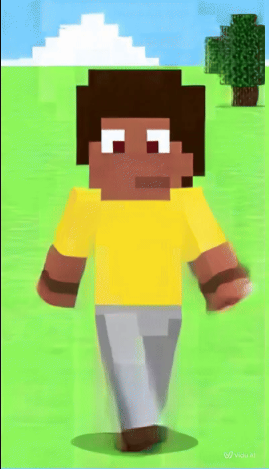
\includegraphics[width=0.8\linewidth]{figs/vidu/1grave.png}
        \caption{\small Quadro com deformação grave (perna e mão embaçados)}
        \label{fig:viduDeformacao1Grave}
    \end{subfigure}
    \legend{\small Fonte: Elaborada pela autora, utilizando a ferramenta Vidu.}
\end{figure}


\begin{figure}[htbp]
    \centering
    \caption{\small Quadros do Vídeo 2 (3D) em cada um dos níveis de deformação}
    \label{fig:viduNiveisDeformacao2}
    \begin{subfigure}{0.32\linewidth}
        \centering
        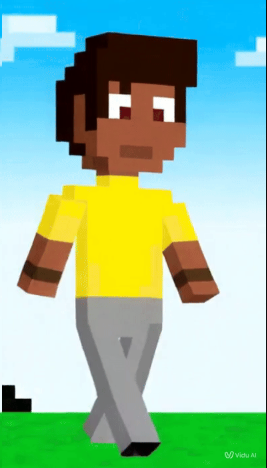
\includegraphics[width=0.9\linewidth]{figs/vidu/2sem.png}
        \caption{\small Quadro classificado como sem deformação}
        \label{fig:viduDeformacao2Sem}
    \end{subfigure}
    \begin{subfigure}{0.32\linewidth}
        \centering
        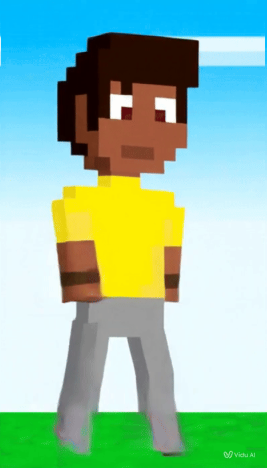
\includegraphics[width=0.9\linewidth]{figs/vidu/2leve.png}
        \caption{\small Quadro com deformação leve (perna e bracelete levemente borrados)}
        \label{fig:viduDeformacao2Leve}
    \end{subfigure}
    \begin{subfigure}{0.32\linewidth}
        \centering
        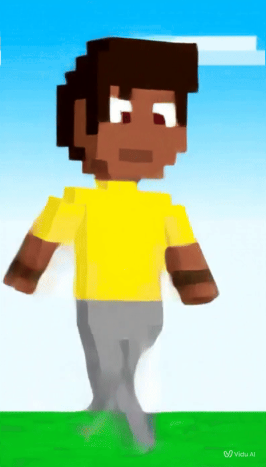
\includegraphics[width=0.9\linewidth]{figs/vidu/2grave.png}
        \caption{\small Quadro com deformação grave (perna deformada, olhos e braços levemente embaçados)}
        \label{fig:viduDeformacao2Grave}
    \end{subfigure}
    \legend{\small Fonte: Elaborada pela autora, utilizando a ferramenta Vidu.}
\end{figure}


\begin{figure}[htbp]
    \centering
    \caption{\small Quadros do Vídeo 3 (2D) em cada um dos níveis de deformação}
    \label{fig:viduNiveisDeformacao3}
    \begin{subfigure}{0.32\linewidth}
        \centering
        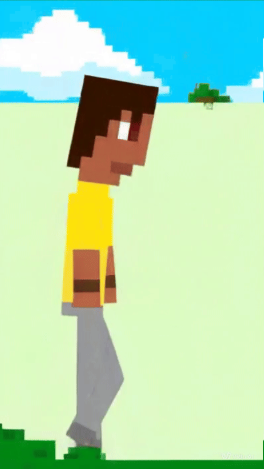
\includegraphics[width=1\linewidth]{figs/vidu/3sem.png}
        \caption{\small Quadro classificado como sem deformação}
        \label{fig:viduDeformacao3Sem}
    \end{subfigure}
    \begin{subfigure}{0.32\linewidth}
        \centering
        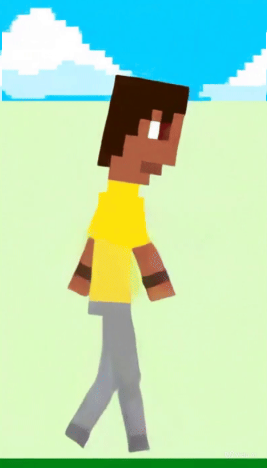
\includegraphics[width=1\linewidth]{figs/vidu/3leve.png}
        \caption{\small Quadro com deformação leve (borda da perna com pequenas ondulações )}
        \label{fig:viduDeformacao3Leve}
    \end{subfigure}
    \begin{subfigure}{0.32\linewidth}
        \centering
        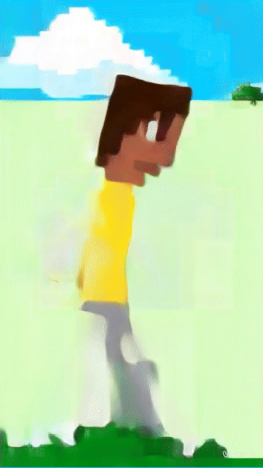
\includegraphics[width=1\linewidth]{figs/vidu/3grave.png}
        \caption{\small Quadro com deformação grave (rosto e corpo borrados, sem braços)}
        \label{fig:viduDeformacao3Grave}
    \end{subfigure}
    \legend{\small Fonte: Elaborada pela autora, utilizando a ferramenta Vidu.}
\end{figure}


O aumento de deformações no resultado 2D possui duas causas prováveis: ou a estrutura do prompt menos restritiva (sem usar a tag como sujeito) resultou em maior instabilidade, ou a ferramenta Vidu possui uma dificuldade em manter a qualidade quadro a quadro ao gerar animações 2D, sendo mais otimizada para a manipulação de referências em 3D.

A interação completa dessa primeira bateria de testes pode ser consultada na Figura \ref{fig:vidu1} no Apêndice \ref{ap.telasIA}.

Para tentar corrigir os erros encontrados nos vídeos, uma segunda bateria de testes foi realizada. Desta vez, foi utilizada como imagem de referência o melhor sprite em side view disponível até o momento (Figura \ref{fig:viduPabloChatGPTSide}). A expectativa era que, ao fornecer uma imagem já na perspectiva correta, a IA teria menos dificuldade em gerar uma animação 2D consistente, sem causar erro na direção e dimensão, além de apresentar um sprite mais adequado.

Os resultados\footnote{\url{https://drive.google.com/drive/folders/1oUOF8-v87bZVZkrv7cTRFy0qcgdaMPZL?usp=sharing}} confirmaram parcialmente a expectativa, eliminando em maior parte o problema da geração em 3D. Entretanto, eles introduziram novos erros. A movimentação do personagem tornou-se ainda mais imprecisa, com a IA adicionando novas ações como pular e girar (Figura \ref{fig:viduGirar}), e fazendo o personagem sair da tela (Figura \ref{fig:viduSair}). Ao modificar a proporção da geração de vídeo, com o objetivo do personagem ter mais espaço para se movimentar sem sair do enquadramento, o sprite passou a deslizar horizontalmente de maneira imprevisível. Ademais, em um dos casos, de forma contraintuitiva, adicionar a palavra 2D ao prompt resultou em uma animação 2D que se tornava 3D ao final (Figura \ref{fig:vidu2D3D}). 


\begin{figure}[htbp]
    \centering
    \begin{minipage}{0.45\textwidth}
    \centering
    \caption{\small Frame do personagem girando para outra direção}
    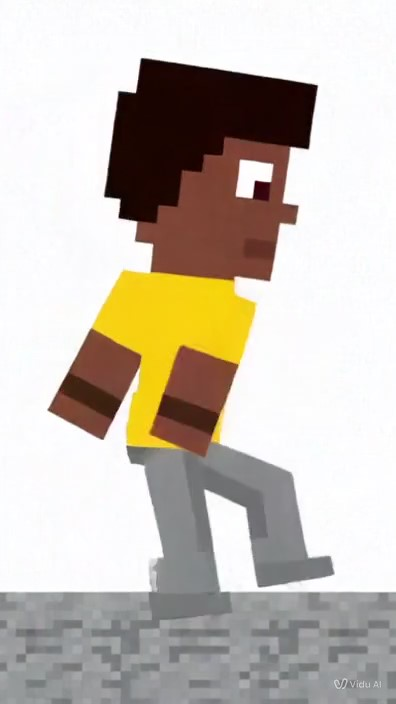
\includegraphics[width=0.6\linewidth]{figs/vidu/frameGirar.jpg}
    \label{fig:viduGirar}
    \legend{\small Fonte: Elaborada pela autora, utilizando a ferramenta Vidu.}
    \end{minipage}\hfill
    \begin{minipage}{0.45\textwidth}
    \centering
    \caption{\small Frame do personagem saindo da tela}    
    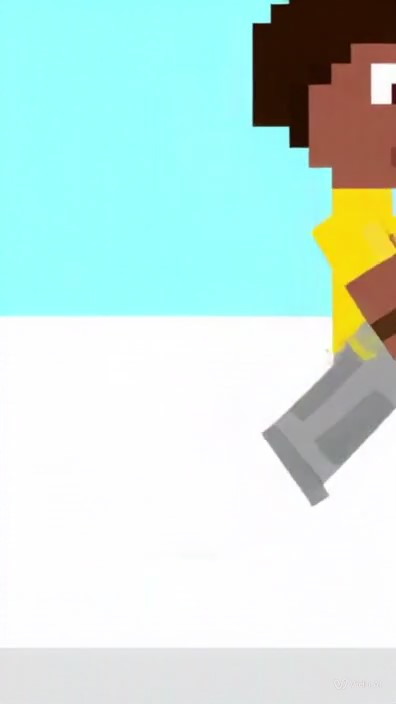
\includegraphics[width=0.6\linewidth]{figs/vidu/frameSairTela.jpg}
    \label{fig:viduSair}
    \legend{\small Fonte: Elaborada pela autora, utilizando a ferramenta Vidu.}
    \end{minipage}\hfill
\end{figure}

\begin{figure}[htbp]
    \centering
    \caption{\small Frame do vídeo gerado em 3D após adicionar a palavra 2D no prompt no Vidu}
    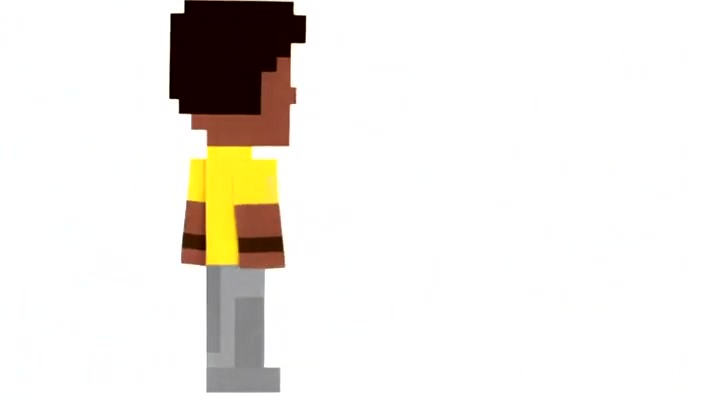
\includegraphics[width=0.5\linewidth]{figs/vidu/frame5_3D.jpg}
    \label{fig:vidu2D3D}
    \legend{\small Fonte: Elaborada pela autora, utilizando a ferramenta Vidu.}
\end{figure}\hfill

Nessa segunda bateria de testes, foi possível gerar um resultado em 2D utilizando a tag da imagem como sujeito do prompt. Mesmo assim, a animação ainda apresentou a inconsistência no movimento, o que indica que a estrutura anterior de prompt não foi a causa dessa instabilidade.

Numa tentativa de corrigir um dos erros que se manteve em praticamente todos os resultados nessa ferramenta, a presença de uma paisagem ao fundo que dificulta o processo de extrair apenas a animação, foi solicitado um vídeo com fundo transparente (utilizando a tag da imagem como sujeito). O resultado gerado foi uma animação 3D, que manteve o movimento de andar na direção incorreta.

A interação completa pode ser consultada nas Figuras \ref{fig:vidu2} a \ref{fig:vidu5} no Apêndice \ref{ap.telasIA}.

Para aprofundar a análise e confirmar a hipótese sobre a dificuldade da ferramenta com o 2D, a mesma análise quantitativa de deformação nos quadros foi replicada nos novos vídeos. 

\begin{table}[htbp]
    \centering
    \caption{Análise quantitativa de frames com deformação, comparando testes com referência em front e side view.}
    \label{tab:viduDeformacoesCompleta}
    \resizebox{\textwidth}{!}{% Redimensiona a tabela para caber na largura da página
    \begin{tabular}{l c c | c c c c c}
        \toprule
        & \multicolumn{2}{c|}{\textbf{Front View como referência}} & \multicolumn{5}{c}{\textbf{Side View como referência}} \\
        \textbf{Nível de deformação} & \textbf{Vídeo 2 (3D)} & \textbf{Vídeo 3 (2D)} & \textbf{Vídeo 1a (2D)} & \textbf{Vídeo 1b (2D)} & \textbf{Vídeo 2 (2D/3D)} & \textbf{Vídeo 3 (2D)} & \textbf{Vídeo 4 (3D)} \\
        \midrule
        Deformação grave (\%) & \textbf{12,2}\% & 36,6\% & 17,1\% & 22,0\% & 26,8\% & 48,8\textbf{\%} & \textbf{12,2}\% \\
        (Frames) & \textbf{5} & 15 & 7 & 9 & 11 & 20 & \textbf{5} \\
        \midrule
        Deformação leve (\%) & 41,5\% & 39,0\% & 56,1\% & 63,4\% & 56,1\% & 34,1\% & 48,8\% \\
        (Frames) & 17 & 16 & 23 & 26 & 23 & 14 & 20 \\
        \midrule
        Sem deformação (\%) & \textbf{46,3\%} & 24,4\% & 26,8\% & 14,6\% & 17,1\% & 17,1\% & \textbf{39,0\%} \\
        (Frames) & \textbf{19} & 10 & 11 & 6 & 7 & 7 & \textbf{16} \\
        \bottomrule
    \end{tabular}
    }
    \legend{\small Fonte: Elaborada pela autora.}
\end{table}

A Tabela \ref{tab:viduDeformacoesCompleta} apresenta os dados de ambas as baterias de testes, permitindo uma comparação direta e reforçando a hipótese de que as deformações são decorrentes da dificuldade da ferramenta com a geração de uma animação 2D, não tendo relação direta com a maneira em que o prompt é estruturado. Primeiramente, observa-se que todos os vídeos gerados em 2D, independentemente da imagem de referência e da estrutura de prompt, apresentam uma taxa de deformação grave e um número de frames sem deformação significativamente piores do que qualquer um dos vídeos gerados em 3D. Embora o uso de uma referência em side view tenha melhorado a estabilidade em alguns casos (Vídeo 1a na Tabela \ref{tab:viduDeformacoesCompleta}), a qualidade geral permaneceu baixa e outros erros sempre estavam presentes.

Outro fator observado foi que no vídeo 2 da segunda bateria de testes, dos 11 frames com deformação grave, apenas 2 deles eram em 3D. Enquanto isso, dos 7 frames sem deformação, 5 deles eram em 3D. Isso mostra que até mesmo durante o mesmo vídeo, a qualidade melhorou no momento em que a animação se tornou 3D.

Crucialmente, como já foi comentado, nesta segunda bateria de testes foi possível gerar um resultado em 2D (nomeado como Vídeo 3 na Tabela \ref{tab:viduDeformacoesCompleta}) utilizando a tag da imagem como sujeito. O fato de a animação ainda assim apresentar a maior taxa de deformação de todos os testes (48,8\%) invalida a hipótese de que a estrutura do prompt era a causa principal da falha. A evidência agora aponta de forma mais conclusiva para a segunda hipótese: a ferramenta Vidu possui uma dificuldade em manter a consistência e a qualidade ao gerar animações em 2D.